\documentclass[a4paper,12pt]{article}

\usepackage[a4paper,left=25mm,right=25mm,bottom=25mm,top=25mm]{geometry}

\usepackage{hyperref}
\usepackage{float}
\usepackage{color}
\usepackage[style=numeric]{biblatex}
\addbibresource{references.bib}
\usepackage{multirow}
\usepackage{makecell}
\usepackage{threeparttable}
\usepackage{bm}
\usepackage{mathtools, nccmath}
\usepackage{amsmath,amsfonts}
\usepackage{algorithmic}
\usepackage{algorithm}
\usepackage{array}
\usepackage[caption=false,font=scriptsize,labelfont=sf,textfont=sf]{subfig}
\usepackage{textcomp}
\usepackage{stfloats}
\usepackage{url}
\usepackage{verbatim}
\setlength{\parindent}{0em}
\setlength{\parskip}{0.5em}
\usepackage{graphicx}
\hyphenation{op-tical net-works semi-conduc-tor IEEE-Xplore}

\begin{document}

\title{Weekly Report}
\author{Zhenyu Zhou}
\maketitle

\section{Finger Knuckle Project}
\subsection{Using histogram equalization to normalize image}
I have tried linear, log, and histogram to normalize image for getting better bounding box detection. From experiments, I found histogram equalization algorithm can get the best performance for detecting finger knuckle on the dark light.


\begin{figure}[ht!]
    \centering
    \subfloat[]{
        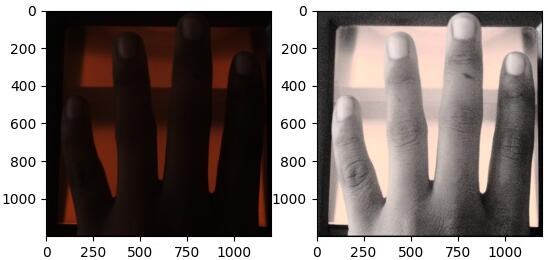
\includegraphics[width=2in]{Figure/18-11-2022/histogram_1.jpg}
        \label{}
    }
    \subfloat[]{
        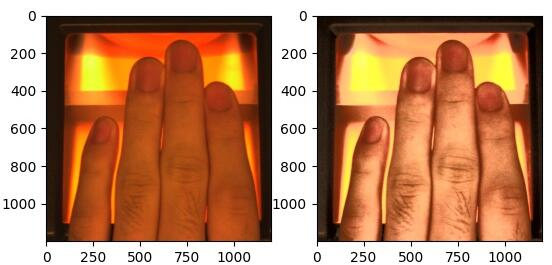
\includegraphics[width=2in]{Figure/18-11-2022/histogram_2.jpg}
        \label{}
    }

    \subfloat[]{
        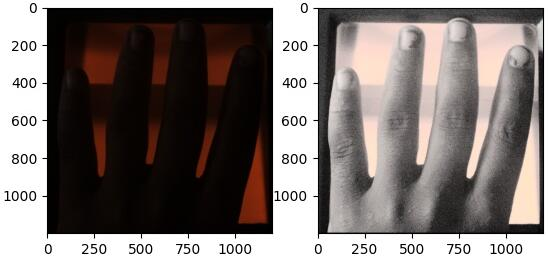
\includegraphics[width=2in]{Figure/18-11-2022/histogram_3.jpg}
        \label{}
    }
    \subfloat[]{
        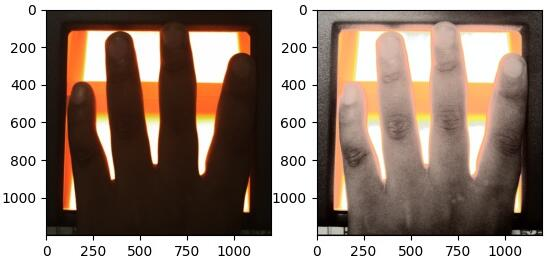
\includegraphics[width=2in]{Figure/18-11-2022/histogram_4.jpg}
        \label{}
    }

    \caption{After using histogram equalization algorithm, the texture of finger knuckle is very clear for detecting.}
    \label{histogram}
\end{figure}

\subsection{Choose the hyperparameters}
\subsubsection{Input image size}
I have tried that change the input image size $h\times w$ from $128\times128$ to $208\times184$. As for the former size, it just follows the RFN model parameter, and the latter input image size is the mean size of the segmented finger knuckle. When I train the RFN model, I also removed the values of ten pixels on each side of the finger knuckle for eliminating background interference. I just used the RFN to test the performance on the middle finger knuckle of left hand, as shown the Table \ref{image_size}. \textcolor{red}{From the result, when compare to the $208\times184$, the $128\times128$ can get better performance. Although the difference of performance is very little, the rest experiments are based on the input $128\times128$ with all-to-all protocol.}


\begin{table}[h]
    \centering
    \caption{Verification performance under different input image size}
    \begin{tabular}{cccccccc}
    \hline
    Protocol                                                                             & Size    & \multicolumn{2}{c}{Left-Little}                                                                            & \multicolumn{2}{c}{Left-Ring}                                                                              & \multicolumn{2}{c}{Left-Index}                                                                             \\ \hline
                                                                                         &         & EER             & \begin{tabular}[c]{@{}c@{}}GAR\\       @ \\      FAR$10^{-4}$\end{tabular} & EER             & \begin{tabular}[c]{@{}c@{}}GAR\\       @ \\      FAR$10^{-4}$\end{tabular} & EER             & \begin{tabular}[c]{@{}c@{}}GAR\\       @ \\      FAR$10^{-4}$\end{tabular} \\ \hline
    \multirow{2}{*}{\begin{tabular}[c]{@{}c@{}}Leave\\One-Out\end{tabular}} & \textbf{128x128} & \textbf{3.34\%} & \textbf{79.00\%}                                                                         & \textbf{0.84\%} & \textbf{97.00\%}                                                                         & \textbf{2.00\%} & \textbf{85.00\%}                                                                         \\
                                                                                         & 208x184 & 4.17\%          & 79.00\%                                                                                  & 1.00\%          & 97.00\%                                                                                  & 2.00\%          & 79.00\%                                                                                  \\ \hline
    \multirow{2}{*}{\begin{tabular}[c]{@{}c@{}}All-to-All\end{tabular}}    & \textbf{128x128} & \textbf{8.19\%} & \textbf{52.00\%}                                                                         & \textbf{2.67\%} & \textbf{84.00\%}                                                                         & \textbf{4.92\%} & \textbf{64.00\%}                                                                         \\
                                                                                         & 208x184 & 10.08\%         & 49.00\%                                                                                  & 3.04\%          & 83.00\%                                                                                  & 6.00\%          & 60.00\%                                                                                  \\ \hline
    \end{tabular}
    \label{image_size}
\end{table}

\subsubsection{The hard margin of triplet loss}
The hard margin will affect the triplet loss to push negative samples away positive samples (probe). But if the hard margin too large, the loss will hard to converge or the model will overfitting. On the contrary, the network cannot be adequately trained result in bad performance on testing set. During training, I change the hard margin on the range of [5, 10, 15, 20, 25, 30, 35, 40], as shown on the Table \ref{triplet-hard-margin}. \textcolor{red}{It can be obviously noticed when $alpha=10$ the $GAR @ FAR = 10^{-4}$ can get the highest values. So in the next section, I will modify hard margin parameter around this value.}

\begin{table}[h]
    \centering
    \caption{Triplet loss with different hard margin}
    \begin{tabular}{ccccccc}
    \hline
    $\alpha$ & \multicolumn{2}{c}{Left-Little}                                                                            & \multicolumn{2}{c}{Left-Ring}                                                                              & \multicolumn{2}{c}{Left-Index}                                                                             \\ \hline
          & EER             & \begin{tabular}[c]{@{}c@{}}GAR\\       @ \\      FAR=$10^{-4}$\end{tabular} & EER             & \begin{tabular}[c]{@{}c@{}}GAR\\       @ \\      FAR=$10^{-4}$\end{tabular} & EER             & \begin{tabular}[c]{@{}c@{}}GAR\\       @ \\      FAR=$10^{-4}$\end{tabular} \\ \hline
    5     & 8.83\%          & 40.00\%                                                                                  & 2.50\%          & 79.00\%                                                                                  & 5.00\%          & 63.00\%                                                                                  \\
    10    & 8.50\%          & \textbf{56.00\%}                                                                         & 2.33\%          & \textbf{86.00\%}                                                                         & 4.17\%          & \textbf{76.00\%}                                                                         \\
    15    & 9.67\%          & 55.00\%                                                                                  & 2.54\%          & 81.00\%                                                                                  & 4.85\%          & 65.00\%                                                                                  \\
    20    & 8.19\%          & 52.00\%                                                                                  & 2.67\%          & 84.00\%                                                                                  & 4.91\%          & 64.00\%                                                                                  \\
    25    & \textbf{7.67\%} & 54\%                                                                                     & 2.67\%          & 76\%                                                                                     & 4.97\%          & 64\%                                                                                     \\
    30    & 9.08\%          & 50\%                                                                                     & \textbf{1.76\%} & 79\%                                                                                     & \textbf{4.00\%} & 55\%                                                                                     \\
    35    & 10.02\%         & 35\%                                                                                     & 2.67\%          & 52\%                                                                                     & 5.36\%          & 47\%                                                                                     \\
    40    & 10.92\%         & 48\%                                                                                     & 2.83\%          & 79\%                                                                                     & 5.58\%          & 64\%                                                                                     \\ \hline
    \end{tabular}
    \label{triplet-hard-margin}
\end{table}

\subsubsection{The hard margin of quadruplet loss}
Because the triplet loss function only focus on the distance between probe images and negative images, the inter-class will ignore by some extent. For increasing intra-class variance and discreasing inter-class variance, the quadruplet loss using four samples (anchor, positive, negative, negative2). But the quadruplet loss has two hard margin, the first one alpha is same as triplet loss while the alpha2 is relative weak. \textcolor{red}{From the Table \ref{quadruplet-hard-margin}, the performance will not have huge different, even the triplet loss can get the best performance on the index finger knuckle of left hand. As for the rest finger knuckle, the performance are similar. When I calculate the triplet, within the same subject, I choose the sample with the greatest distance from the anchor as the positive. For the negative, I compare it with all the samples of the other two subjects and choose the one with the smallest distance.}

\begin{table}[h]
    \centering
    \caption{Quadruplet loss with different hard margin}
    \begin{tabular}{llllllll}
    \hline
    $\alpha$ & $\alpha$2 & \multicolumn{2}{l}{Left-Little}                                                                            & \multicolumn{2}{l}{Left-Ring}                                                                              & \multicolumn{2}{l}{Left-Index}                                                                             \\ \hline
          &        & EER             & \begin{tabular}[c]{@{}l@{}}GAR\\       @ \\      FAR=10\textasciicircum{}-4\end{tabular} & EER             & \begin{tabular}[c]{@{}l@{}}GAR\\       @ \\      FAR=10\textasciicircum{}-4\end{tabular} & EER             & \begin{tabular}[c]{@{}l@{}}GAR\\       @ \\      FAR=10\textasciicircum{}-4\end{tabular} \\ \hline
    10    & 0      & 8.50\%          & 56.00\%                                                                                  & 2.33\%          & 86.00\%                                                                                  & \textbf{4.17\%} & \textbf{76.00\%}                                                                         \\
    10    & 5      & 8.75\%          & 56.00\%                                                                                  & 2.42\%          & 79.00\%                                                                                  & 4.92\%          & 60.00\%                                                                                  \\
    10    & 10     & 8.75\%          & 55.00\%                                                                                  & 2.92\%          & 72.00\%                                                                                  & 5.33\%          & 60.00\%                                                                                  \\
    10    & 15     & 8.83\%          & \textbf{61.00\%}                                                                         & 2.17\%          & \textbf{90.00\%}                                                                         & 5.08\%          & 72.00\%                                                                                  \\
    20    & 5      & 8.58\%          & 59.00\%                                                                                  & 1.86\%          & 86.00\%                                                                                  & 4.50\%          & \textbf{75.00\%}                                                                         \\
    20    & 10     & \textbf{8.17\%} & 59.00\%                                                                                  & \textbf{1.50\%} & 81.00\%                                                                                  & \textbf{3.92\%} & 70.00\%                                                                                  \\
    20    & 15     & 10.92\%         & 45.00\%                                                                                  & 2.50\%          & 82.00\%                                                                                  & 5.75\%          & 61.00\%                                                                                  \\
    20    & 20     & 8.69\%          & \textbf{66.00\%}                                                                         & 1.70\%          & \textbf{89.00\%}                                                                         & 5.10\%          & 63.00\%                                                                                  \\
    30    & 15     & \textbf{7.50\%} & 59.00\%                                                                                  & \textbf{1.54\%} & 76.00\%                                                                                  & 4.75\%          & 58.00\%                                                                                  \\
    40    & 20     & 9.08\%          & 58.00\%                                                                                  & 2.09\%          & 86.00\%                                                                                  & 5.00\%          & 70.00\%                                                                                  \\ \hline
    \end{tabular}
    \label{quadruplet-hard-margin}
\end{table}

\subsection{Using spatial transformer network to increase RFN performance}
Spatial transformer network (STN) can learn the matrix of homography transform to affine finger knuckle. If the loss higher than a threshold during training process, I freeze the spatial transformer network layer without updating weights. And the STN just output $\begin{bmatrix} 1 & 0 & 0 \\ 0 & 1 & 0 \end{bmatrix}$ matrix. When the loss lower than a threshold, the STN weights can be updated for outputting a transform matrix. \textcolor{red}{When I use the STN module to improve RFN performance, from the Table \ref{stn}, the STN module can improve the RFN model silght}

\begin{table}[h]
    \caption{Peformance of spatial transfomer network based on RFN}
    \begin{tabular}{ccccccccc}
    \hline
    Model   & $\alpha$ & T & \multicolumn{2}{c}{Left-Little}                                                                            & \multicolumn{2}{c}{Left-Ring}                                                                              & \multicolumn{2}{c}{Left-Index}                                                                             \\ \hline
            &     &  & EER             & \begin{tabular}[c]{@{}c@{}}GAR\\       @ \\      FAR=$10^{-4}$\end{tabular} & EER             & \begin{tabular}[c]{@{}c@{}}GAR\\       @ \\      FAR=$10^{-4}$\end{tabular} & EER             & \begin{tabular}[c]{@{}c@{}}GAR\\       @ \\      FAR=$10^{-4}$\end{tabular} \\ \hline
    RFN     & 10 &0   & 8.50\%          & 56.00\%                                                                                  & 2.33\%          & \textbf{86.00\%}                                                                         & 4.17\%          & \textbf{76.00\%}                                                                         \\
    STNRFN & 10  &10  & \textbf{6.92\%} & \textbf{58.00\%}                                                                         & \textbf{1.42\%} & \textbf{86.00\%}                                                                         & 4.92\%          & 60.00\%                                                                                  \\
    RFNSTN & 10 &10   & 8.06\%          & 54.00\%                                                                                  & 2.00\%          & 80.00\%                                                                                  & 3.91\% & 62.00\%              
    \\
    STNRFN & 10 &0   & \textbf{6.832\%}          & 49.00\%                                                                                  & 1.50\%          & 65.00\%                                                                                  & \textbf{3.334\%} & 61.00\%           
    \\
    ResSTN  & 10 &NA   & 8.42\%          & 40.00\%                                                                                  & 2.09\%          & 70.00\%                                                                                  & 4.92\% & 48.00\%      
    \\
    ResSTN & 10 &0   & 10.624\%          & 45.00\%                                                                                  & 2.25\%          & 84.00\%                                                                                  & 5.29\% & 70.00\%                                                                     \\ \hline
    \end{tabular}
    \label{stn}
\end{table}

\subsection{Using Rotation and Shift Invariant loss to train RFN model}
Above experiments are based on the MSE loss function to train model, then I use the RSIL loss function to replace the MSE loss function to test the performance. From the below Table

\begin{table}[h]
    \caption{Peformance of RSIL loss based on RFN}
    \begin{tabular}{ccccccccc}
    \hline
    Model   & $\alpha$  & \multicolumn{2}{c}{Left-Little}                                                                            & \multicolumn{2}{c}{Left-Ring}                                                                              & \multicolumn{2}{c}{Left-Index}                                                                             \\ \hline
            &      & EER             & \begin{tabular}[c]{@{}c@{}}GAR\\       @ \\      FAR=$10^{-4}$\end{tabular} & EER             & \begin{tabular}[c]{@{}c@{}}GAR\\       @ \\      FAR=$10^{-4}$\end{tabular} & EER             & \begin{tabular}[c]{@{}c@{}}GAR\\       @ \\      FAR=$10^{-4}$\end{tabular} \\ \hline
    RFN-MSE     & 10    & 8.50\%          & 56.00\%                                                                                  & 2.33\%          & 86.00\%                                                                      & 4.17\%          & 76.00\%                                                                         \\
    RFN-RSIL & 10    & \textbf{6.34\%} & \textbf{58.00\%}                                                                         & \textbf{1.08\%} & \textbf{96.00\%}                                                                         & \textbf{2.834\%}          & \textbf{87\%}                                                                                                                                     \\ \hline
    \end{tabular}
    \label{rsil}
\end{table}

\begin{figure}[ht!]
    \centering
    \subfloat[]{
        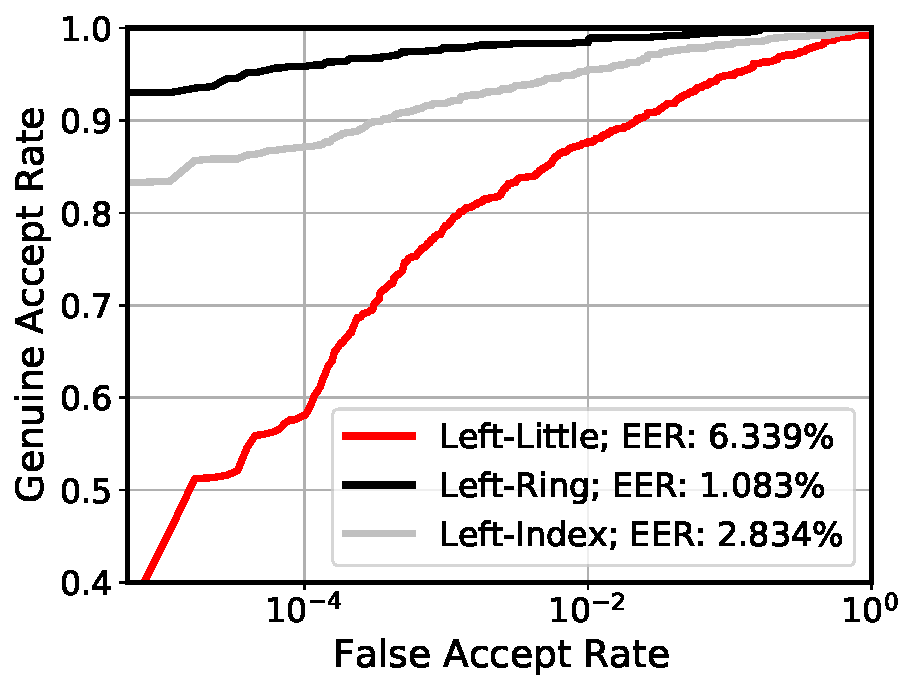
\includegraphics[width=2in]{Figure/18-11-2022/roc.pdf}
        \label{}
    }

    \caption{Comprative mathing performance with ROC cure on the littler finger knuckle, ring finger knuckle, and index finger knuckle of left hand.}
    \label{rfn-rsil}
\end{figure}

\subsubsection{Data augmentation}
\begin{table}[h]
    \centering
    \caption{Data augmentation}
    \begin{tabular}{cccc}
    \hline
    Augmentation & Parameter & Augmentaion & Parameter \\ \hline
    hsv\_h       & 0.015     & shear       & NA        \\
    hsv\_s       & 0.7       & perspective & NA        \\
    hsv\_v       & 0.4       & flipud      & NA        \\
    degrees      & 10         & fliplr      & NA        \\
    translate    & 0.1       & mosaic      & NA        \\
    scale        & 0.1       & mixup       & NA        \\ \hline
    \end{tabular}
    \label{data-augmentation}
\end{table}
From the Table \ref{data-augmentation}, I used the left part data augmentation algorithm, because the right part algorithm will totally change the finger knuckle texture which cannot be solved by RFN-RSIL model. Meanwhile, the RFN-RSIL model gets the best performance form above experiments, therefore, I continue to use the RFN-RSIL model. \textcolor{red}{The model is still be trained, so I cannot show any performance result at here.}

\subsection{Find the best score fusion parameter}
\subsubsection{Dynamic fusion}
\begin{equation}
    fusion\_score = w\times knuckle\_score + (1-w)\times print\_score
\end{equation}
\textcolor{red}{I have changed the $w$ from 0 to 1, the step size is 0.05, and I can get the best fusion score when $w$ equal to 0.35.} I mainly tried on the little finger and ring finger of left hand. From the 

\begin{figure}[ht!]
    \centering
    \subfloat[]{
        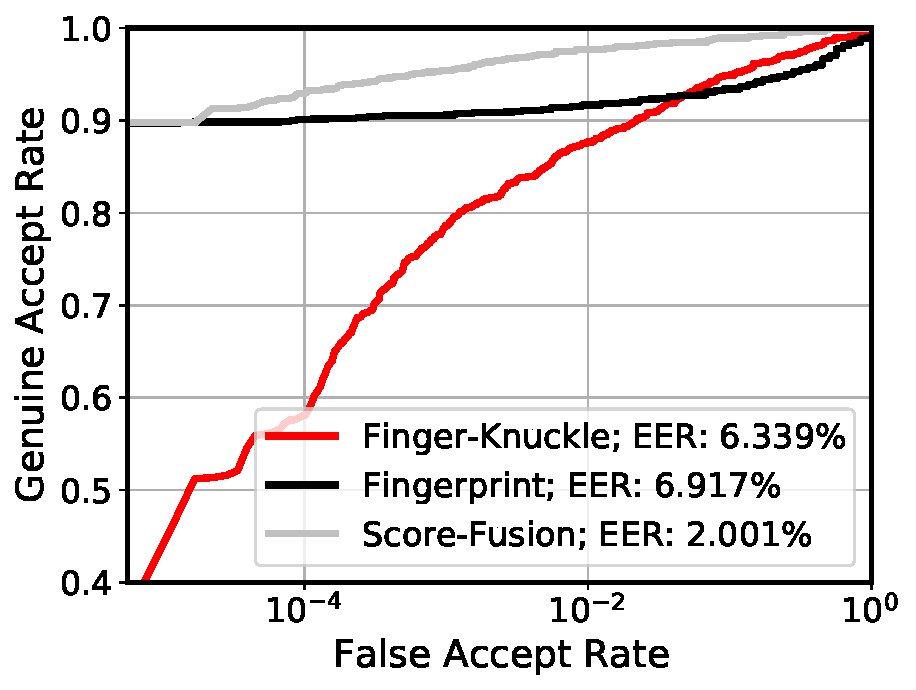
\includegraphics[width=2in]{Figure/18-11-2022/dynamic_score_01.pdf}
        \label{}
    }
    \subfloat[]{
        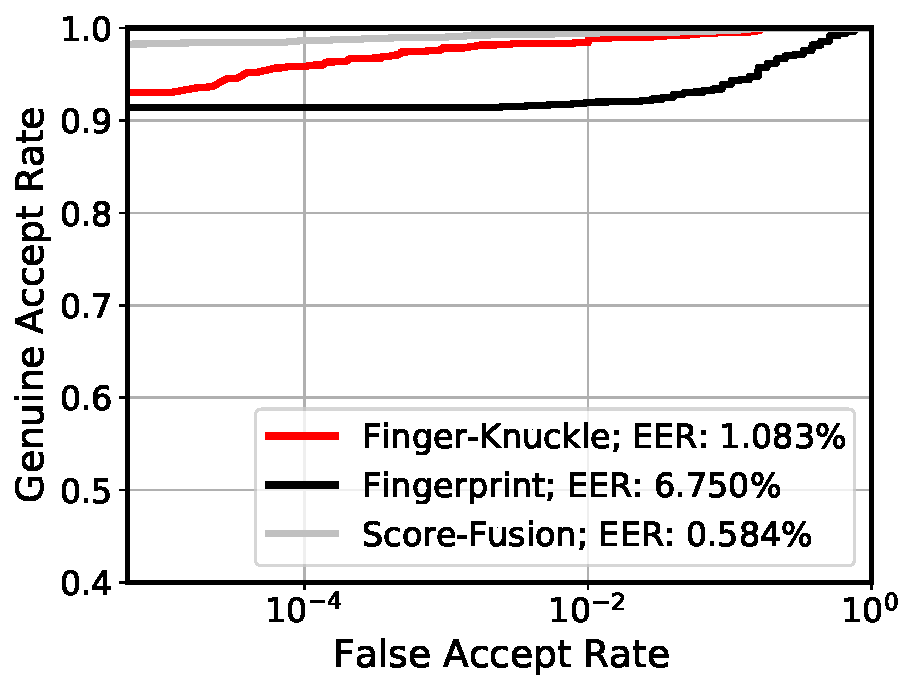
\includegraphics[width=2in]{Figure/18-11-2022/dynamic_score_02.pdf}
        \label{}
    }

    \caption{When the $w$ equal to 0.35, the dynamic fusion score algorithm can get the best matching performance on the (a)little finger of left hand (b) ring finger of left hand. }
    \label{dynamic-score}
\end{figure}

\subsubsection{Holistic Fusion}
\begin{equation}
    fusion\_score = (w\times knuckle\_score + (1-w) \times print\_score) \times (1 + 1 / (2 - knuckle\_score))
\end{equation}
I also changed the $w$ from 0 to 1 with step size 0.05 on the Equation (2). From the Fig. \ref{holistic} and Fig. \ref{dynamic-score}, their performance is same from the ROC curve.
\begin{figure}[ht!]
    \centering
    \subfloat[]{
        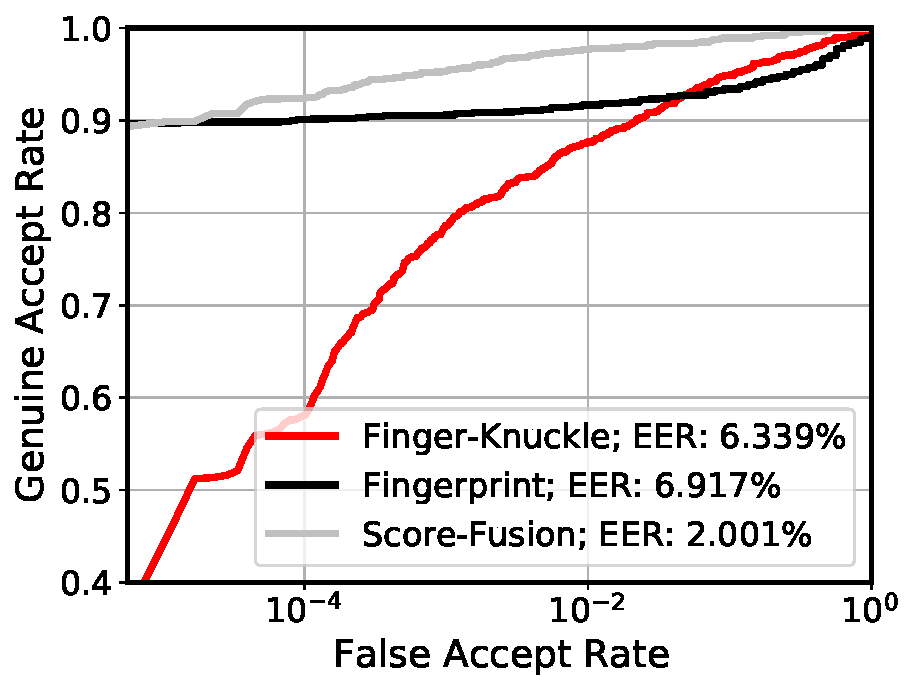
\includegraphics[width=2in]{Figure/18-11-2022/holistic_score_01.pdf}
        \label{}
    }
    \subfloat[]{
        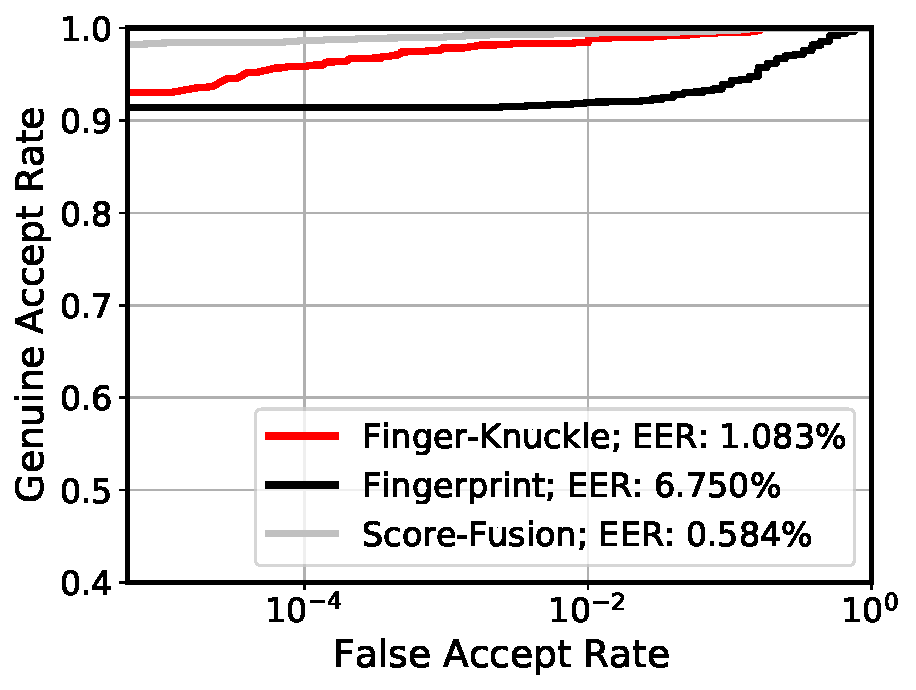
\includegraphics[width=2in]{Figure/18-11-2022/holistic_score_02.pdf}
        \label{}
    }

    \caption{When the $w$ equal to 0.2, the holistic fusion score algorithm can get the best matching performance on the (a)little finger of left hand (b) ring finger of left hand. }
    \label{holistic}
\end{figure}

\subsubsection{Nonlinear Fusion}
\begin{equation}
    fusion\_score = ((1 + print)/(1 + knuckle))^{\alpha} \times (1 + knuckle)^2
\end{equation}
As for the nonlinear fusion method, we can change the $\alpha$ from 1 to 2, then I use $0.05$ step size to change the parameter. When the $alpha$ is 1.45, then the nonlinear fusion method can get the best performance, from the Fig. \ref{nonlinear}. \textcolor{red}{From only test on the little finger and ring finger of left hand, the nonlinear fusion method is the best.}

\begin{figure}[ht!]
    \centering
    \subfloat[]{
        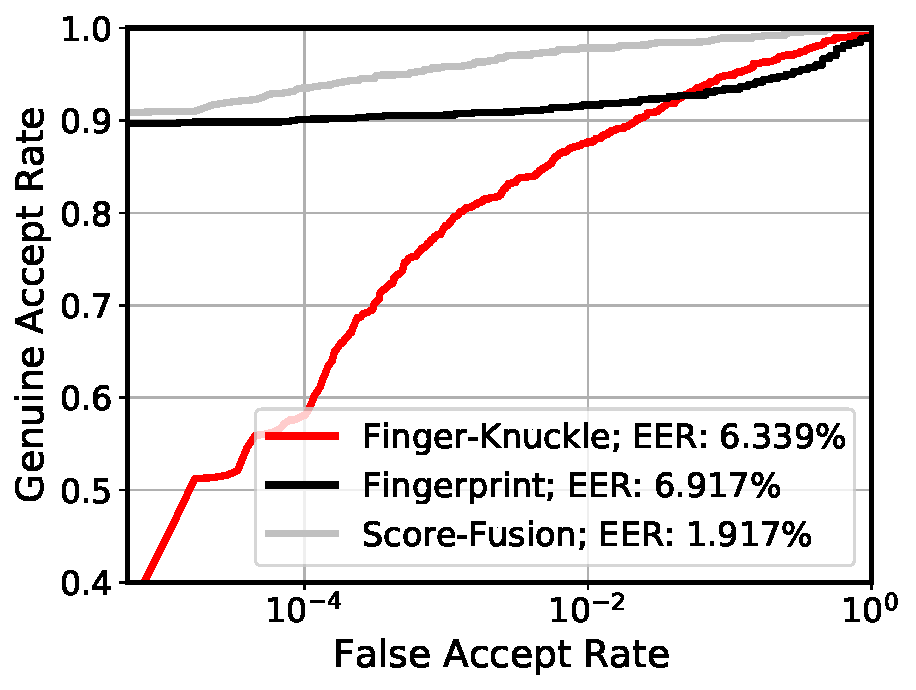
\includegraphics[width=2in]{Figure/18-11-2022/nonlinear_score_01.pdf}
        \label{}
    }
    \subfloat[]{
        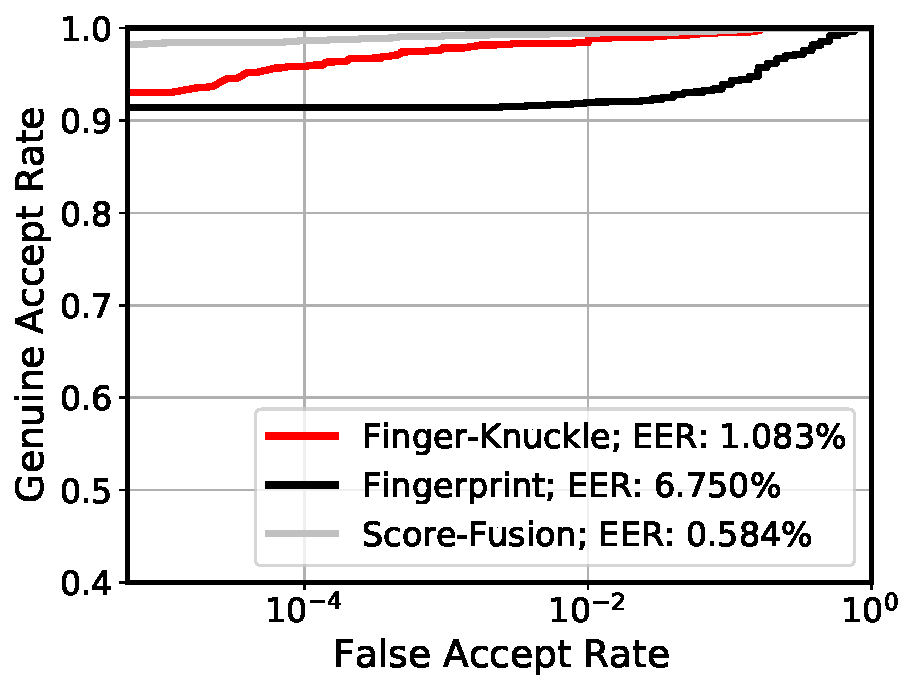
\includegraphics[width=2in]{Figure/18-11-2022/nonlinear_socre_02.pdf}
        \label{}
    }

    \caption{When the $w$ equal to 0.45, the holistic fusion score algorithm can get the best matching performance on the (a)little finger of left hand (b) ring finger of left hand. }
    \label{nonlinear}
\end{figure}


% \section{References}

\printbibliography[heading = none ]


\end{document}